%!TEX root = paper.tex
\subsection{Solitary wave on a simple beach}
This is an analytic testcase and a laboratory experiment conducted at the California Institute of Technology, Pasadena, California. A linear solitary (better called single) wave propagates over a  constant bathymetry, until it reaches a linear sloping beach, s.t. the wave inundates the dry area and the offtake takes place after the wave has reached the maximum runup point. 
The experimental data include the surface elevation measured at different points in time for a non-breaking and a breaking wave. The analytic testcase considers only a non-breaking wave, but yields comparison data in terms of time series as well as data at two locations.
The experimental data serve for validation of the models concerning their ability to model inundation. Additionally to the experimental data, a linear analytic solution is provided, s.t. verification of our models is also tested.

The initial condition is prescribed as a linear analytic solitary wave solution (similar to the one in section \ref{sec:B_compositebeach})
\begin{align}
\xi(\bx,t)&=a \ \text{cosh}^{-2}(K(x-ct-x_0)), \\
u(\bx,t)&=-c\frac{\xi(\bx,t)}{d},
\end{align}
with the initial actual amplitude $a$, propagation velocity $c=\csw$ with scale factor $K=\sqrt{\left(\frac{3a}{4d^3}\right)}$ and displacement $x_0=X_0+L=d \, \text{cot}(\beta)+\text{arccos}(\sqrt{20})\frac{1}{Kd}$, with $\beta=\text{arccot}(19.85)$. The entire domain length is $L=48 \, \text{m}$. The simulation time is $40$ seconds. 

In the analytic testcase, the ratio between amplitude and depth is $\frac{a}{d}=0.019$, whereas the laboratory experiment uses  $\frac{a}{d}=0.0185$. 
For breaking waves in the laboratory experiment, the ratio between amplitude and depth is $\frac{a}{d}=0.3$. We choose $d=1$m and $a$ accordingly.
We impose reflecting boundary conditions at the boundary in x-direction and periodic boundary conditions in y-direction. For the setup see figure \ref{fig:simplebeach_setup}. 

\begin{figure}[htbp]
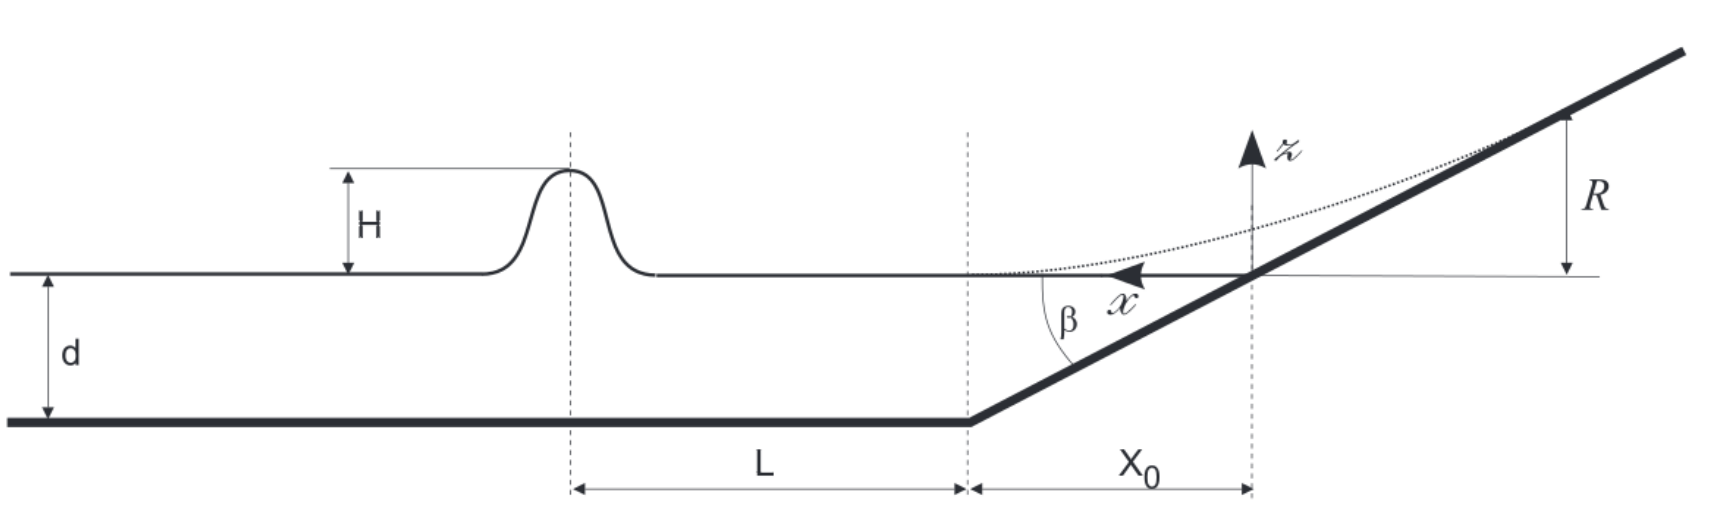
\includegraphics[width=\textwidth]{simplebeach_setup}
\caption{Setup of the testcase solitary wave on a simple beach. (Letters do not fit to text decription.)}
\label{fig:simplebeach_setup}
\end{figure}

\subsubsection{Results of \nh\ model}
Figures \eqref{fig:nh_simplebeach_ana_nh_Nhy} display the comparison of the nonlinear SWE with the linear analytic solution. The first five figures present simulation results at required time steps, whereas the sixth figure shows the comparison at two positions over time.
The models results compared to the analytic solution are prone to oszillations, especially close to the shoreline. 

Need to improve, and also tested only with Lhy.
Add maximal runup and convergence test.
\begin{figure}[htbp]
\begin{minipage}{\textwidth}
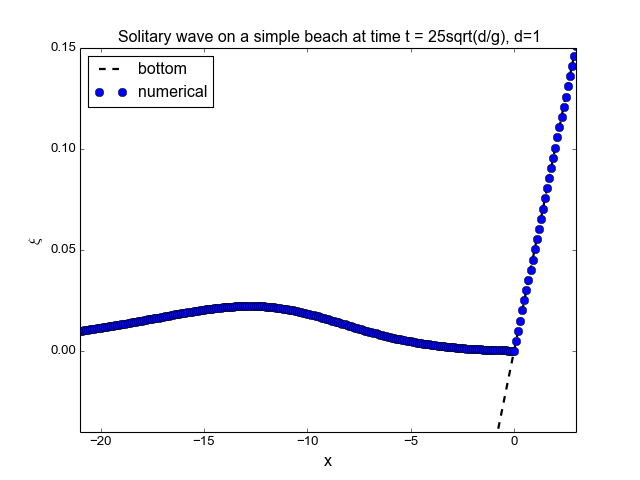
\includegraphics[width=0.48\textwidth]{simplebeach_ana_t=25tau_nh_Nhy}
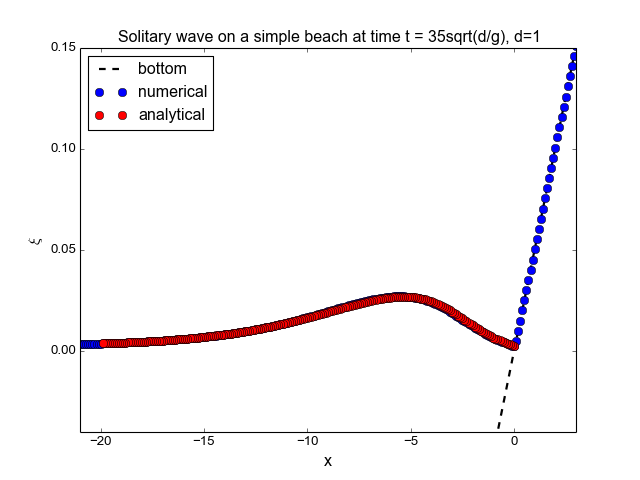
\includegraphics[width=0.48\textwidth]{simplebeach_ana_t=35tau_nh_Nhy}
\end{minipage} \\
\begin{minipage}{\textwidth}
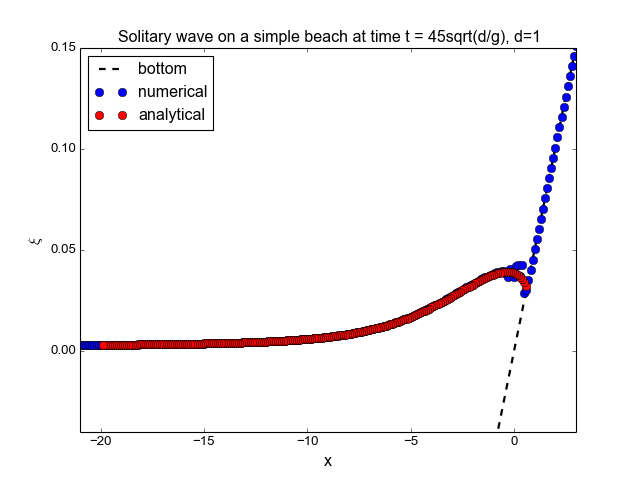
\includegraphics[width=0.48\textwidth]{simplebeach_ana_t=45tau_nh_Nhy}
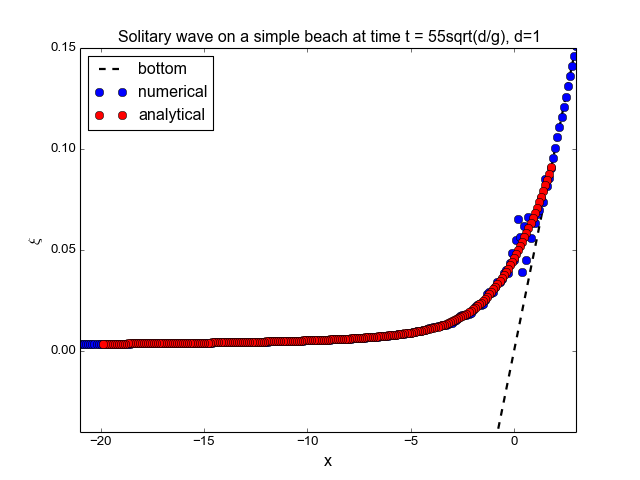
\includegraphics[width=0.48\textwidth]{simplebeach_ana_t=55tau_nh_Nhy}
\end{minipage} \\
\begin{minipage}{\textwidth}
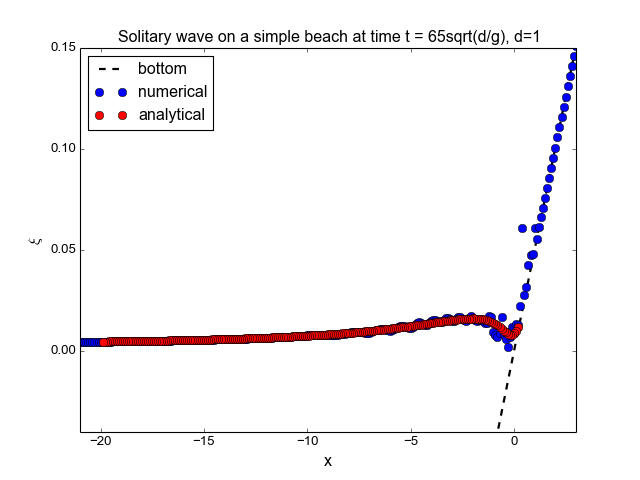
\includegraphics[width=0.48\textwidth]{simplebeach_ana_t=65tau_nh_Nhy}
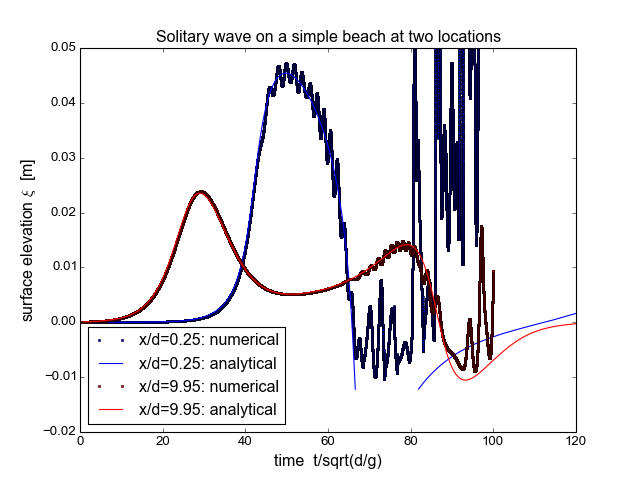
\includegraphics[width=0.48\textwidth]{simplebeach_ana_x_nh_Nhy}
\end{minipage}
\caption{Comparison of the linear analytical (red) sea surface height of the
solitary wave with the simulation results of the \nh\ model in its version of nonlinear shallow water equations (blue). (The x-axis values should be multiplied by (-1), and colors changed.)}
\label{fig:nh_simplebeach_ana_nh_Nhy}
\end{figure}
